\section{Comentários sobre o Código}
\begin{verbatim}
%(pnrz.m)
%Geração de um pulso retangular de largura T
%Uso da função: pout=pnrz(T);
%definição da função
function pout=prect(T);
%pout é um vetor de 1's de tamanho T
pout = ones(1,T);
end

%(prz.m)
%Geração de um pulso retangular de largura T/2
%Uso da função: pout = prz(T);
%definição da função:
function pout=prz(T);
%pout é um vetor com T/4 zeros, seguido de T/2 1's, seguido de T/4 zeros
pout = [zeros(1,T/4) ones(1, T/2) zeros(1, T/4)];
end

%(psine.m)
%geração de um pulso senoidal de largura T
%definição da função:
function pout=psine(T)
%pout é um vetor igual ao seno de pi*(T de 0 a T-1)/T
pout = sin(pi*[0:T-1]/T);
end

%(prcos.m)
%Uso: y=prcos(rollfac,lenght,T)
%definição da função:
function y=prcos(rollfac,lenght, T)
%rollfac = 0 a 1 é o fator de roll off
%lenght é a largura onesided do pulso no número de T
%lenght = 2T + 1;
%T é a taxa de sobreamostragem
%rcosfir gera um filtro de cosseno levantado de acordo com os argumentos
y=rcosfir(rollfac,lenght,T,1,'normal');
end

%(binary_eye.m)
%Geração e Plotagem de Diagramas de Olho
%limpar as variáveis e a tela atual de figura
clear;clf;
data = sign(randn(1,400)); % gerar 400 bits randomizados

%geração de 400 pontos de ruído com variância r
%r = 0.01;
%ruid = randn(1,400)*sqrt(r);
%data = data + ruid

Tau = 64; %definir o período de símbolo
% gerar trem de impulsos inserindo Tau-1 zeros entre cada bit
dataup = upsample(data, Tau) 
yrz = conv(dataup, prz(Tau)); %Sinal polar RZ, conv é a operação convolução
yrz = yrz(1:end-Tau+1); %retirar a "cauda" do vetor yrz
ynrz = conv(dataup, pnrz(Tau)); %Sinal polar NRZ
ynrz = ynrz(1:end-Tau+1); %Retirar a "cauda" do vetor ynrz
ysine = conv(dataup,psine(Tau)); %Meia Senóide Polar
ysine = ysine(1:end-Tau+1); %Retirar a "cauda" do vetor ysine
Td=4; %definição de Td
yrcos=conv(dataup, prcos(0.5,Td,Tau)); 

%cosseno levantado truncado em 4 períodos com rolloff =0.5
yrcos=yrcos(2*Td*Tau:end-2*Td*Tau+1); %Gerando trem de pulsos

%geração do diagama de olho RZ
eye1=eyediagram(yrz,2*Tau,Tau,Tau/2); title('RZ eye-diagram'); 

%geração do diagrama de olho NRZ
eye2=eyediagram(ynrz,2*Tau,Tau,Tau/2); title('NRZ eye-diagram'); 

%geração do diagrama de olho Meia-Senóide
eye3=eyediagram(ysine, 2*Tau, Tau, Tau/2); title=('Half-Sine eye-diagram'); 

%geração do diagrama de olho Cosseno-Levantado
eye4=eyediagram(yrcos,2*Tau,Tau); title('Raised-Cosine eye-diagram');

%(Mary_eye.m)
%Geração de Diagrama de Olho e Plotagem (PAM Quaternário)
%limpar as variáveis e telas de figura
clear;clf;
%geração de 400 símbolos PAM quaternário (valores possíveis: -1,-3, 1, 3) 
data = sign(randn(1,400)) +2*sign(randn(1,400));

%geração de 400 pontos de ruído com variância r
%r = 0.01;
%ruid = randn(1,400)*sqrt(r);
%data = data + ruid

%definição do período de símbolo
Tau=64;
% gerar trem de impulsos inserindo Tau-1 zeros entre cada bit
dataup = upsample(data, Tau) 
yrz = conv(dataup, prz(Tau)); %Sinal polar RZ, conv é a operação convolução
yrz = yrz(1:end-Tau+1); %retirar a "cauda" do vetor yrz
ynrz = conv(dataup, pnrz(Tau)); %Sinal polar NRZ
ynrz = ynrz(1:end-Tau+1); %Retirar a "cauda" do vetor ynrz
ysine = conv(dataup,psine(Tau)); %Meia Senóide Polar
ysine = ysine(1:end-Tau+1); %Retirar a "cauda" do vetor ysine
Td=4; %definição de Td
yrcos=conv(dataup, prcos(0.5,Td,Tau)); 

%cosseno levantado truncado em 4 períodos com rolloff =0.5
yrcos=yrcos(2*Td*Tau:end-2*Td*Tau+1); %Gerando trem de pulsos

%geração do diagama de olho RZ
eye1=eyediagram(yrz,2*Tau,Tau,Tau/2); title('RZ eye-diagram'); 

%geração do diagrama de olho NRZ
eye2=eyediagram(ynrz,2*Tau,Tau,Tau/2); title('NRZ eye-diagram'); 

%geração do diagrama de olho Meia-Senóide
eye3=eyediagram(ysine, 2*Tau, Tau, Tau/2); title=('Half-Sine eye-diagram'); 

%geração do diagrama de olho Cosseno-Levantado
eye4=eyediagram(yrcos,2*Tau,Tau); title('Raised-Cosine eye-diagram');

\end{verbatim}

\section{Degradações}
\subsection{Ruído Branco}
O ruído branco AWGN pode ser gerado simplesmente através da função randn(), que gera uma distribuição normal, podemos gerar um vetor R=randn(1,400)*sqrt(r), adicionando este vetor ao vetor de dados gerado podemos enxergar qual a contribuição do ruído no diagrama de olho para um determinado r, que é a variância, neste caso escolhemos r=0.01 de forma a não fechar completamente o diagrama, mas ainda mostrar um pouco do "fechamento".
\section{Diagramas de olho}
\pagebreak


\begin{figure}
\centering
\begin{minipage}{.5\textwidth}
  \centering
  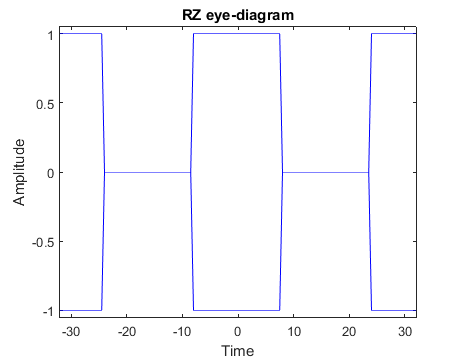
\includegraphics[width=\linewidth]{DolhoRZsrb.png}
  \captionof{figure}{RZ Binário sem ruído}
  \label{fig:test5}
\end{minipage}%
\begin{minipage}{.5\textwidth}
  \centering
  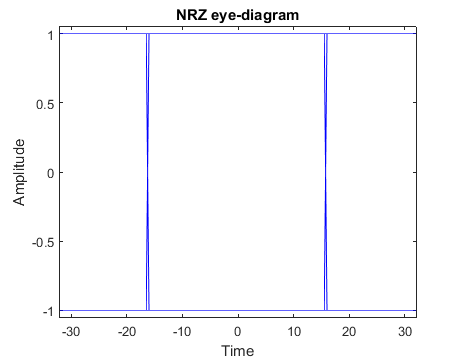
\includegraphics[width=\linewidth]{DolhoNRZsrb.png}
  \captionof{figure}{NRZ Binário sem ruído}
  \label{fig:test6}
\end{minipage}
\end{figure}

\begin{figure}
\centering
\begin{minipage}{.5\textwidth}
  \centering
  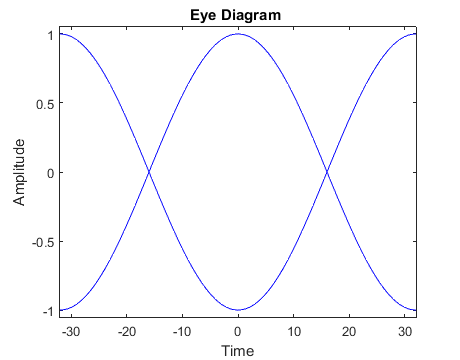
\includegraphics[width=\linewidth]{Dolhosensrb.png}
  \captionof{figure}{Meia Senóide Binário sem ruído}
  \label{fig:test7}
\end{minipage}%
\begin{minipage}{.5\textwidth}
  \centering
  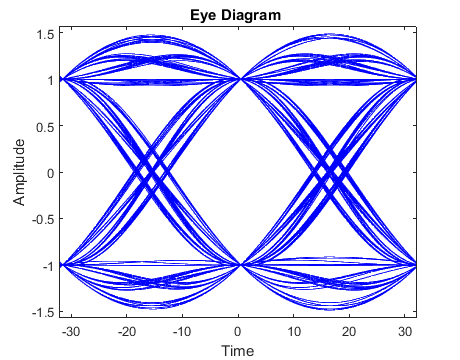
\includegraphics[width=\linewidth]{Dolhoclsrb.png}
  \captionof{figure}{Cosseno Levantado Binário sem ruído}
  \label{fig:test8}
\end{minipage}
\end{figure}


\begin{figure}
\centering
\begin{minipage}{.5\textwidth}
  \centering
  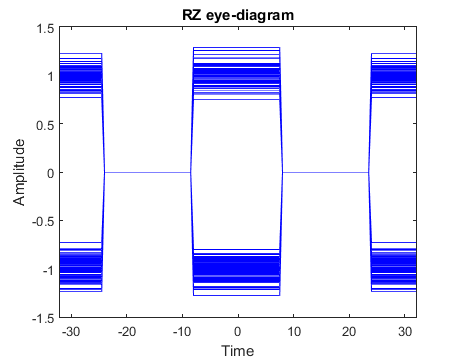
\includegraphics[width=\linewidth]{DolhoRZcrb.png}
  \captionof{figure}{RZ Binário com ruído}
  \label{fig:test9}
\end{minipage}%
\begin{minipage}{.5\textwidth}
  \centering
  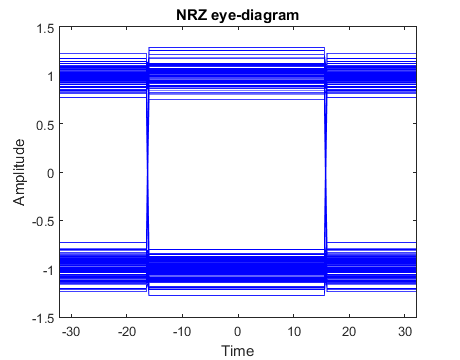
\includegraphics[width=\linewidth]{DolhoNRZcrb.png}
  \captionof{figure}{NRZ Binário com ruído}
  \label{fig:test10}
\end{minipage}
\end{figure}

\begin{figure}
\centering
\begin{minipage}{.5\textwidth}
  \centering
  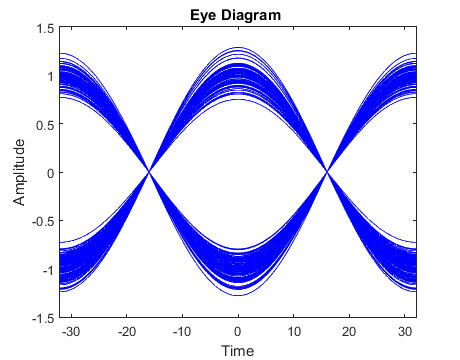
\includegraphics[width=\linewidth]{Dolhosencrb.png}
  \captionof{figure}{Meia Senóide Binário com ruído}
  \label{fig:test11}
\end{minipage}%
\begin{minipage}{.5\textwidth}
  \centering
  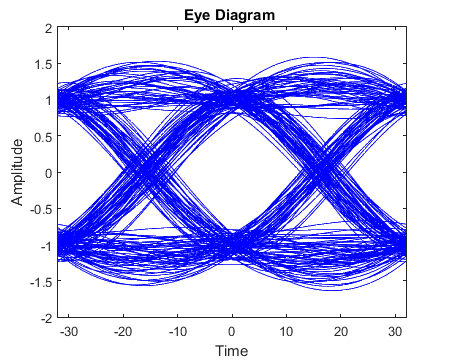
\includegraphics[width=\linewidth]{Dolhoclcrb.png}
  \captionof{figure}{Cosseno Levantado Binário com ruído}
  \label{fig:test12}
\end{minipage}
\end{figure}


\begin{figure}
\centering
\begin{minipage}{.5\textwidth}
  \centering
  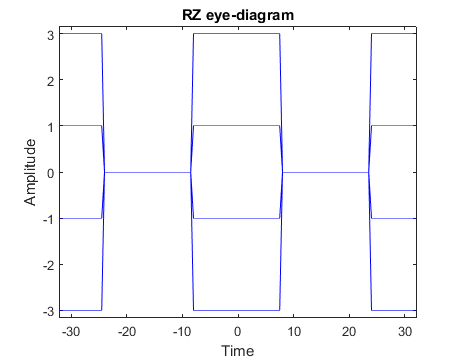
\includegraphics[width=\linewidth]{DolhoRZsrq.png}
  \captionof{figure}{RZ Quaternário sem ruído}
  \label{fig:test13}
\end{minipage}%
\begin{minipage}{.5\textwidth}
  \centering
  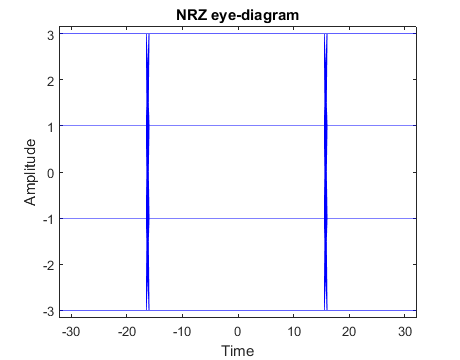
\includegraphics[width=\linewidth]{DolhoNRZsrq.png}
  \captionof{figure}{NRZ Quaternário sem ruído}
  \label{fig:test14}
\end{minipage}
\end{figure}

\begin{figure}
\centering
\begin{minipage}{.5\textwidth}
  \centering
  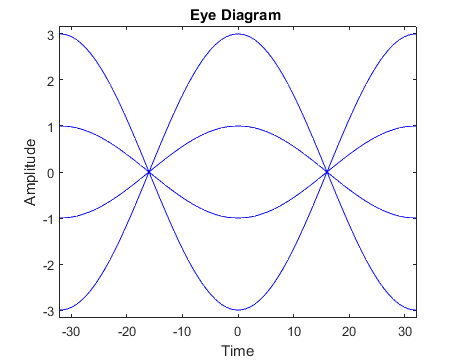
\includegraphics[width=\linewidth]{Dolhosensrq.png}
  \captionof{figure}{Meia Senóide Quaternário sem ruído}
  \label{fig:test15}
\end{minipage}%
\begin{minipage}{.5\textwidth}
  \centering
  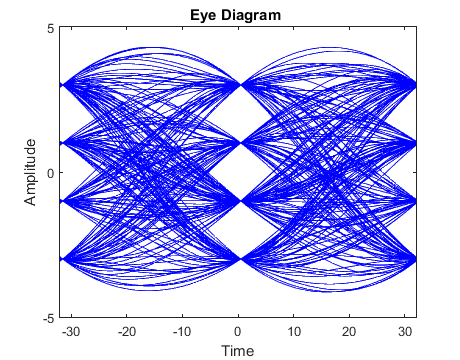
\includegraphics[width=\linewidth]{Dolhoclsrq.png}
  \captionof{figure}{Cosseno Levantado Quaternário sem ruído}
  \label{fig:test16}
\end{minipage}
\end{figure}


\begin{figure}
\centering
\begin{minipage}{.5\textwidth}
  \centering
  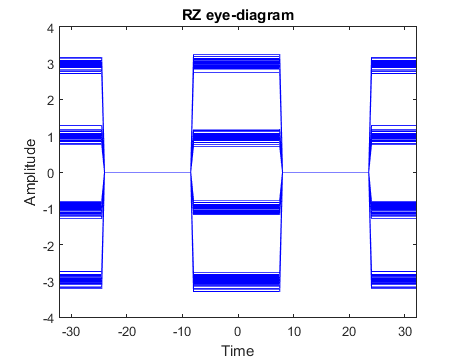
\includegraphics[width=\linewidth]{DolhoRZcrq.png}
  \captionof{figure}{RZ Quaternário com ruído}
  \label{fig:test17}
\end{minipage}%
\begin{minipage}{.5\textwidth}
  \centering
  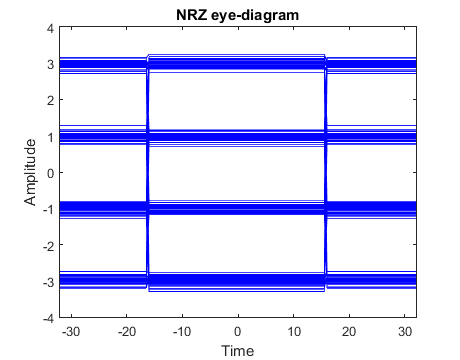
\includegraphics[width=\linewidth]{DolhoNRZcrq.png}
  \captionof{figure}{NRZ Quaternário com ruído}
  \label{fig:test18}
\end{minipage}
\end{figure}

\begin{figure}
\centering
\begin{minipage}{.5\textwidth}
  \centering
  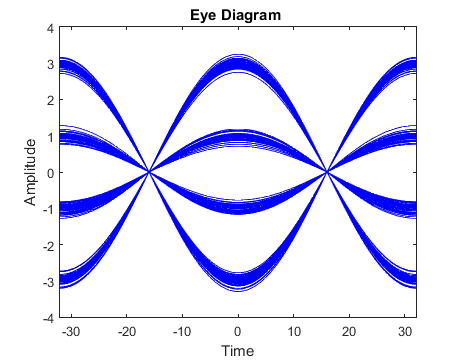
\includegraphics[width=\linewidth]{Dolhosencrq.png}
  \captionof{figure}{Meia Senóide Quaternário com ruído}
  \label{fig:test19}
\end{minipage}%
\begin{minipage}{.5\textwidth}
  \centering
  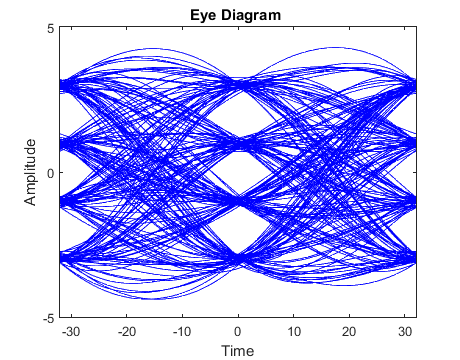
\includegraphics[width=\linewidth]{Dolhoclcrq.png}
  \captionof{figure}{Cosseno Levantado Quaternário com ruído}
  \label{fig:test20}
\end{minipage}
\end{figure}

